\documentclass[10pt,a4paper]{article}
\usepackage[utf8]{inputenc}

\usepackage{amsmath}
\usepackage{amsfonts}
\usepackage{amssymb}
\usepackage{booktabs}
\usepackage{caption}
\usepackage{csquotes}
\usepackage{graphicx}
\usepackage{float}
\usepackage{hyperref}
\usepackage{listings}
\usepackage{siunitx}
\usepackage{svg}
\usepackage{titlesec}
\usepackage{url}
\usepackage{xcolor}

%Beautiful lstlistning
\DeclareCaptionFont{white}{\color{white}}
\DeclareCaptionFormat{listing}{%
 \parbox{\textwidth}{\colorbox{gray}{\parbox{0.95\textwidth}{#1#2#3}}\vskip-4pt}}
\captionsetup[lstlisting]{format=listing,labelfont=white,textfont=white}
\lstset{frame=lrb,xleftmargin=\fboxsep,xrightmargin=0.045\textwidth}

%More sections
\setcounter{secnumdepth}{4}

%Different margin
\usepackage[margin=30mm]{geometry}

%Author and title info
\title{Configurable Radiation Testsuite \\- \\Documentation}
\author{Mattis Jaksch}
\date{\today}

\begin{document}
\maketitle

\tableofcontents

\flushleft

\newpage

\section{Overview}
This testsuite is developed to automate various test procedures, like thermal-vacuum, radiation or just general long-term tests. The use is made to be as easy as possible to have a comprehensive and fast test setup. It offers interfaces to gather all the needed data, together with some measurements to protect the device under test (DUT) and act in unsafe situations.

\bigbreak

The test-suite supports different devices (e.g. power supplies, ethernet clients, data acquisition units, ...) which can be configured to control the process in a desired way. The interaction between components is realized with the \enquote{qt-signal-slot}\footnote{Refer to \url{doc.qt.io/qt-5/signalsandslots.html}} mechanism. One may add signals to a device which are then send out to trigger actions on other devices. A trigger-device can be, for example, a power supply switching off to protect the DUT.

	\subsection{Mainwindow}
	Here in figure \eqref{f:main_menu} an overview on the general program is given. The different options are described in the following sub-chapters.
	
	\begin{figure}[H]
\centering
\includesvg[width=0.9\textwidth]{1_Plain_Expl.svg}
\caption{Main menu of the suite}
\label{f:main_menu}
	\end{figure}
	
	\subsubsection{Top Row}	
	
	On the top row, on the left side, configurations for all the components in the various tabs can be either stored or loaded in a single file. The stored configuration file is also human readable and editable.
	
	\bigbreak
	
	On the right side, the test can be started or stopped. Starting and stopping the test sends a signal to all components. E.g. the power supply will turn selected channels on/off and start/stop the logging. Hence one can not click the start-button twice in a row!
	
	\subsubsection{Mid Row (Run Information)}
	
	In the row below is the run information. To start a run, one should first create a \enquote{New run} by clicking the button and creating a folder to store all the devices log files. On the right of this button, the current file location and the time of the run are displayed. If one stops the run, the time also halts till the run gets restarted. 

	\bigbreak	
	
	The log files are named after the individual components (e.g. \enquote{PSU Left}), so one should make sure to not have any names twice to avoid confusion.
	
	\subsubsection{Tabs}
	
	The tabs contain various devices of the same kind. Currently implemented are:
	
	\begin{itemize}
\item Power-supply
\item Labjack
\item RF (Reception client for the Analog Devices IIO-daemon)\footnote{Deactivated}
\item DIO (Digital I/O to switch relays)\footnote{Not implemented yet}
\item PROG (Starts and external program including arguments; and records the output)
\item ETH (Ethernet data reception)
	\end{itemize}		
	
	\subsection{Testrun}	
	
	\begin{figure}[H]
\centering
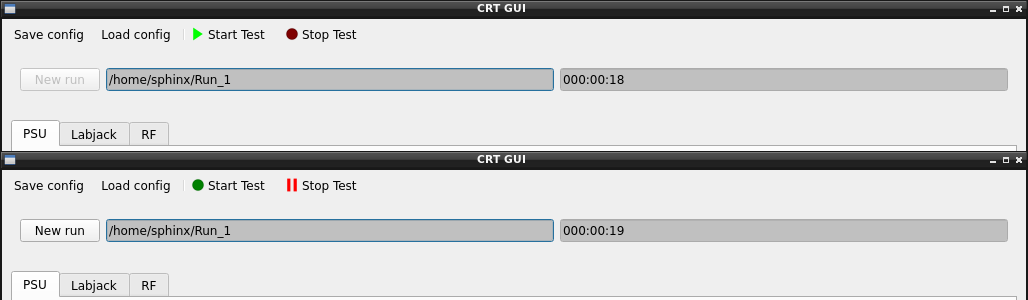
\includegraphics[width=0.9\textwidth]{./4_Testrun.png}
\caption{An active testrun in the suite}
	\end{figure}
	
	If a test run is started, the \enquote{Start Test} button and the \enquote{New run} button get deactivated and the time starts to count up. Meanwhile in the background, logfiles are generated with a UTC timestamp. The data itself is stored in a \textit{.csv} format to be easily readable. To every datapoint or row being stored, a relative timestamp in milliseconds is added.
	
	\bigbreak
	
	To stop the run and therefore also the logging and timer, the \enquote{Stop Test} button should be pressed. After that, a run can also be continued by clicking the \enquote{Start Test} button again.	
	
\newpage
	
\section{Components}
Here the various components, corresponding to the tabs, are explained. The description includes a function overview, an example and two creation procedures (manual / config) as well as the currently supported devices.

	\subsection{Power-Supply}
	The power supply tab controls a given device remotely. An arbitrary maximum voltage / current can be set to avoid unwanted change and damage. In figure \eqref{f:psu_example} an supply example is given. The psu can be easily controlled via voltage and current line edits. Also every channel can be enabled / disabled individually and also by a signal (e.g. with the \enquote{Start Test} / \enquote{Stop Test}). Also, a time-line of the voltage and current is given on a small graph for each channel in steps of 1 second over an interval of 30 seconds. 	
	
	\begin{figure}[H]
\centering
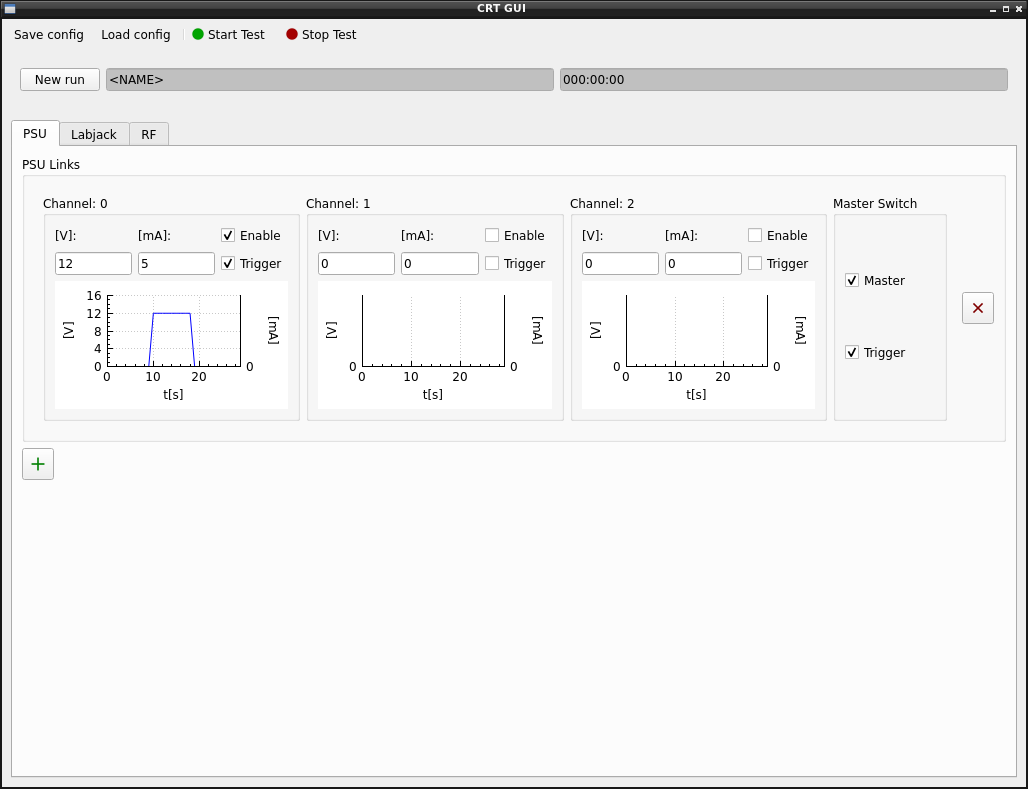
\includegraphics[width=0.9\textwidth]{./2_PSU_example.png}
\caption{An example with a Rohde\&Schwarz 3-channel power supply}
\label{f:psu_example}
	\end{figure}	 
	
	\subsubsection{Manual Creation}	
	\label{c:psu_manual_creation}
	
	The window for manual creation is presented in figure \eqref{f:psu_menu}. In the first row an individual (meaningful) name can be chosen. In the second row the vendor is put in (case insensitive). Then follows the address which has a IPv4 part and a port number after the double dot. In the last three rows, a description of the power supply is given with the number of channels and the maximum voltage/current. The voltage here, as well as the current, can be set to an arbitrary level to avoid accidental overvoltage.
	
	\begin{figure}[H]
	\centering
	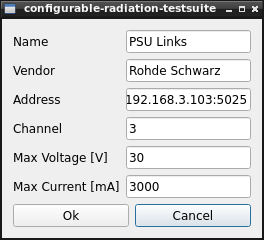
\includegraphics[width=0.4\textwidth]{./2_PSU_menu.png}
	\caption{Creation menu for a power-supply}
	\label{f:psu_menu}
	\end{figure}
	
	\subsubsection{Config Creation}
	
	The power-supply is denoted in the configuration file in the \enquote{PSU} section. The first three lines correspond to the manual creation in chapter \ref{c:psu_manual_creation}. After that, the latest channel settings are brought up. They have a prefix $c$, a number $X$ as identifier and a suffix, with $vs$ for voltage-set, $cs$ current-set, $vm$ voltage-max and $cm$ current-max. Therefore the maximum settings can be defined individually here, in contrast to the manual creation.
	
\begin{lstlisting}[caption=PSU Config]
Section PSU
	name=PSU Links
	address=192.168.3.103:5025
	channel=3
	c0vs=12
	c0cs=500
	c0vm=30
	c0cs=3000
	c1vs=0
	c1cs=0
	c1vm=5
	c1cm=1500
	signal=
EndSection
\end{lstlisting}
	
		\subsubsection{Supported devices}
		Support for other devices can be easily added. One only needs to edit the \textit{psu.*} files and add a few lines for the correct SCPI\footnote{Standard Commands for Programmable Instruments} Code.
	
		\begin{table}[H]
		\centering
		\begin{tabular}{ll}
		\toprule
		Supplier			& Model \\ \midrule
		Rhode\&Schwarz		& HMC8043 \\
		TTI					& (?) \\
		\bottomrule
		\end{tabular}			
		\end{table}	
		
\newpage
	
	\subsection{Labjack}
	The Labjack is a data acquisition device to measure voltages in a range of $\SI{10}{\milli\volt}$ to $\SI{10}{\volt}$. As a consequence, the available resolution is dependant on the chosen measurement range. The same goes for the data rate which depends on the settling time (see low-pass filter) and for the chosen resolution. In the figure \eqref{f:lbj_example} a Labjack with two channels (one differential, one single-ended) are shown. In the top row, the mentioned data-rate, resolution and settling time can be chosen. The \enquote{Maximum} check box allows to set the data-rate to the available maximum. Below presented are the two channels with a boundary (\enquote{0} means \enquote{not set}), their latest value and the chosen gain (only post-processing). At the bottom a graph is presented containing all plotted channels. To display the channels in the graph, they can be switched on or off by the corresponding check box. 
	
	\begin{figure}[H]
	\centering
	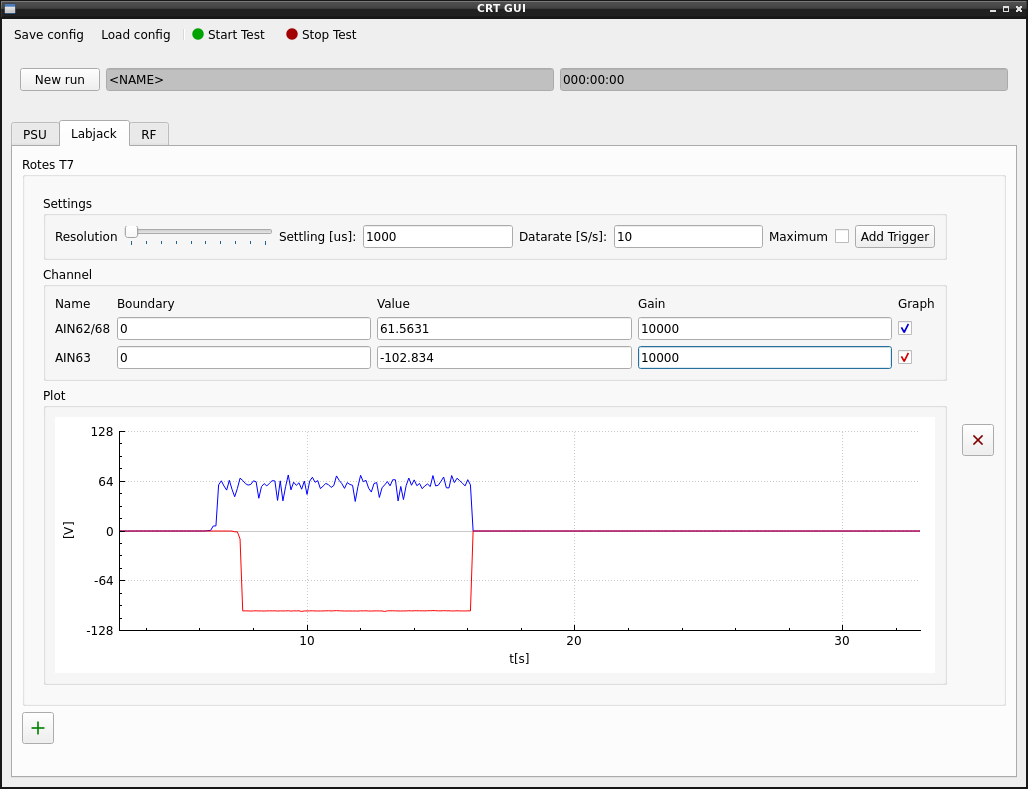
\includegraphics[width=0.9\textwidth]{./3_LBJ_example.png}
	\caption{An example with a T7 Labjack data acquisition device}
	\label{f:lbj_example}
	\end{figure}
	
	\subsubsection{Manual Creation}	
	
	The window for manual creation is presented in figure (\ref{f:lbj_menu}). In the first row an individual name can be chosen. The channel names in the second row can also be chosen individually. The third and fourth row determines the used channels\footnote{Refer to \url{labjack.com/support/datasheets/t-series/ain}} and if they are differential or not. A differential channel is given by a certain positive and negative address, whereas single ended just use $199$ as negative channel.
	
	
	\begin{figure}[H]
	\centering
	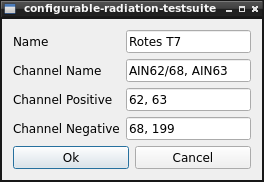
\includegraphics[width=0.4\textwidth]{./3_LBJ_menu.png}
	\caption{Creation menu for a Labjack}
	\label{f:lbj_menu}
	\end{figure}
	
	\subsubsection{Config Creation}	
	The LabJack is denoted in the configuration file in the \enquote{LBJ} section. First the name is defined and after that the number of channels as a validity check. The individual channels are written with a prefix $c$, a number $X$ and their features as suffix:
	
	\begin{itemize}
	\item $n$: Name
	\item $pc$: Positive Channel
	\item $nc$: Negative Channel
	\item $b$: Boundary value
	\item $g$: Gain value
	\end{itemize}
	
\begin{lstlisting}[caption=LBJ Config]
Section LBJ
	name=Rotes T7
	channel=2
	c0n=AIN62/68
	c0pc=62
	c0nc=68
	c0b=0
	c0g=1
	c1n=AIN63
	c1pc=63
	c1nc=199
	c1b=0
	c1g=1
	signal=
EndSection
\end{lstlisting}
	
		\subsubsection{Supported devices}
		To support other devices the addresses in the \textit{Labjack.*} files have to be extended.
	
		\begin{table}[H]
		\centering
		\begin{tabular}{ll}
		\toprule
		Supplier			& Model \\ \midrule
		Labjack				& T7 \\
		\bottomrule
		\end{tabular}			
		\end{table}	

	\newpage
	\subsection{RF Signals - Deactivated}
	\textbf{Due to technical issues, this option is deactivated at the moment!}

	\bigbreak
	
	In order to verify RF signals, the RF tab (see figure \ref{f:rf_example}) can be used. The current implementation supports only sine signals and requires IQ data with 16 bit. An evaluation margin in exponents of 2 can be chosen as an upper / lower boundary. Once this boundary is crossed (and the evaluation is active) an error signal will be emitted.
		
		\begin{figure}[H]
\centering
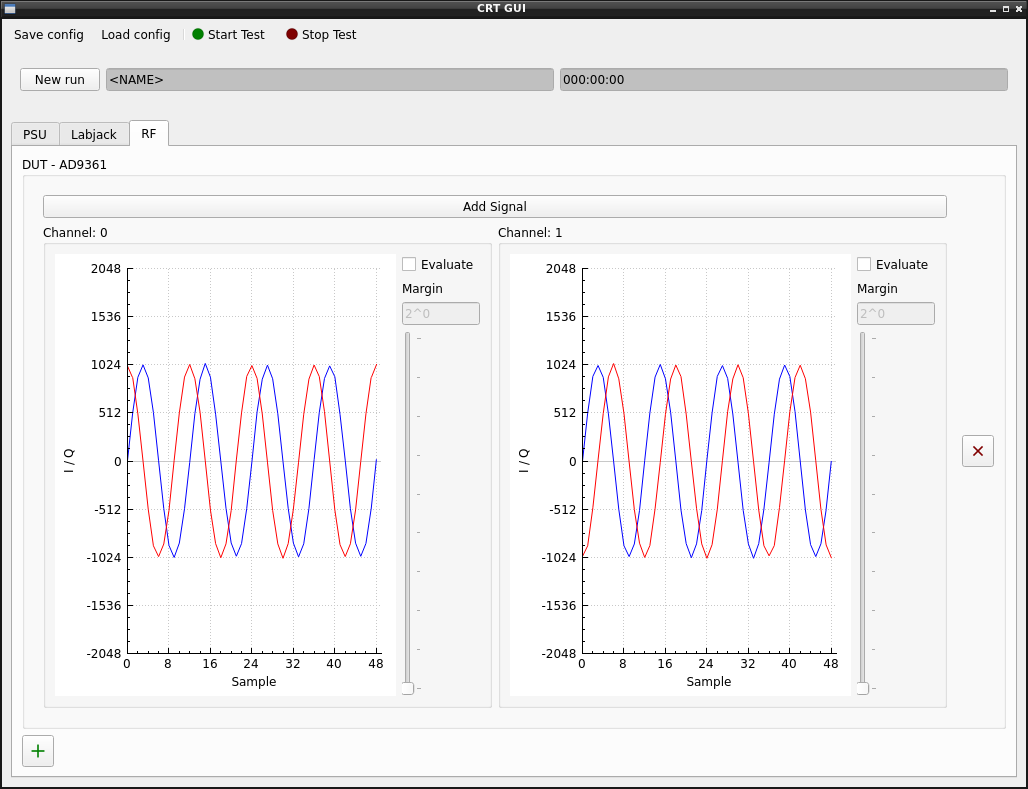
\includegraphics[width=0.9\textwidth]{./6_RF_example.png}
\caption{An active RF testrun in the suite}
\label{f:rf_example}
		\end{figure}
	
		\subsubsection{Manual Creation}
		For the manual creation, refer to figure (\ref{f:rf_menu}). In the first row an individual name can be chosen. The second row contains the IPv4 address including the port number. In the third row the number of channels is specified.		
		
		\begin{figure}[H]
\centering
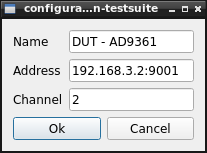
\includegraphics[width=0.4\textwidth]{./6_RF_menu.png}
\caption{RF creation menu}
\label{f:rf_menu}
		\end{figure}
			
		\subsubsection{Config Creation}
				
		The RF is denoted in the configuration file in the \enquote{RF} section. First the name is defined, then the IPv4 address of the device and after that the number of channels. The individual channels are written with a prefix $c$, a number $X$ and their features as suffix:
	
	\begin{itemize}
	\item $m$: margin
	\end{itemize}
	
\begin{lstlisting}[caption=RF Config]
Section RF
	name=DUT - AD9361
	address=192.168.3.2:9001
	channel=2
	c0m=0
	c1m=0
	signal=
EndSection
\end{lstlisting}
	
		\subsubsection{Data Reception}
		The current implementation uses the simple \textit{ncat}\footnote{Refer to \url{de.wikipedia.org/wiki/Netcat}} command to receive raw data over Ethernet. This makes it rather independent. The current data protocol is given in table (\ref{t:rf_data}):
		
		\begin{table}[H]
		\centering
		\begin{tabular}{c|cc|cc|cc|cc}
		\toprule
		2 Channel	& \multicolumn{8}{c}{8 Byte}\\ \midrule
		IQ-Data		& \multicolumn{4}{c|}{4 Byte} & \multicolumn{4}{c}{4 Byte} \\ \hline 
		I	& \multicolumn{2}{c}{2 Byte} & \multicolumn{2}{c|}{2 Byte} & \multicolumn{4}{c}{} \\ 
		Q	& \multicolumn{4}{c|}{} & \multicolumn{2}{c}{2 Byte} & \multicolumn{2}{c}{2 Byte} \\  \hline
		Byte		& LSB & MSB & LSB & MSB & LSB & MSB & LSB & MSB \\ \bottomrule
		\end{tabular}
		\caption{Data structure of the RF IQ-data}
		\label{t:rf_data}
		\end{table}
		
	\newpage
	
	\subsection{Programm}
	To communicate with the DUT in an individual way (or to initialize it), a specified program can be started. This is done in the program tab (see figure \ref{f:prog_example}). Here, the path to a program - one wants to use - can be put in. It can then be either started early manually (and logged) or via the trigger mechanism, together with the rest of the test. So far, only console applications are supported.
	
	Additional to the program, arguments can be added. To pass the current run directory the variable \textit{\$directory} can the be used.
	
	\begin{figure}[H]
	\centering
	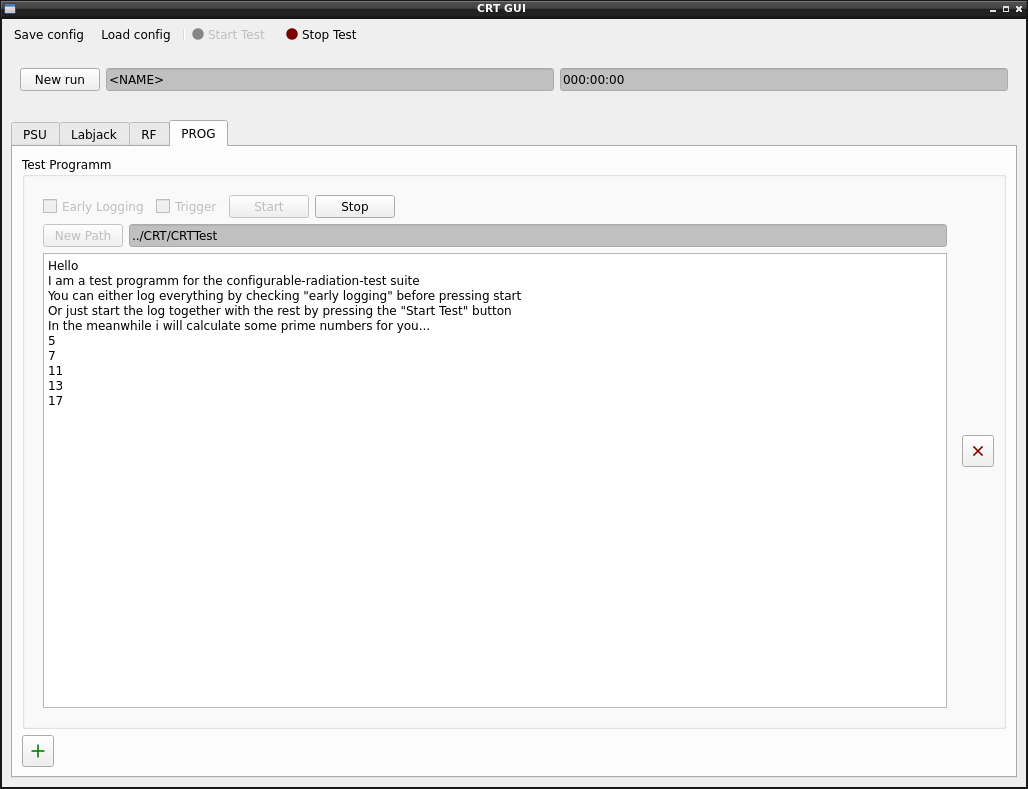
\includegraphics[width=0.9\textwidth]{./7_PROG_example.png}
	\caption{An active PROG testrun in the suite}
	\label{f:prog_example}
	\end{figure}
	
		\subsubsection{Manual Creation}	
		For the manual creation, refer to figure (\ref{f:prog_menu}). In the first row an individual name can be chosen. The path to the program is set in the second row. 
		
		\begin{figure}[H]
\centering
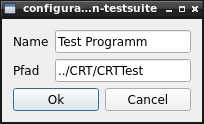
\includegraphics[width=0.4\textwidth]{./7_PROG_menu.png}
\caption{RF creation menu}
\label{f:prog_menu}
		\end{figure}
			
		\subsubsection{Config Creation}
		The program is denoted in the configuration file in the \enquote{PROG} section. First the name is defined, then the path to the program.
	
\begin{lstlisting}[caption=PROG Config]
Section PROG
	name=Test Programm
	path=../CRT/CRTTest
	signal=
EndSection
\end{lstlisting}
	
	\newpage
	\subsection{Ethernet}
	The ethernet port can specify a port to be open for data reception. The name, port number and information on the reception are displayed. In figure \eqref{f:eth_example} an example is given. Once the test starts, the port is opened and data can be received. A timeout can be set to trigger other devices (added via \enquote{Add Signal}). On the right an indicator shows if the connection is (in-)active and lights up if data has been recently received. 
	
	\begin{figure}[H]
\centering
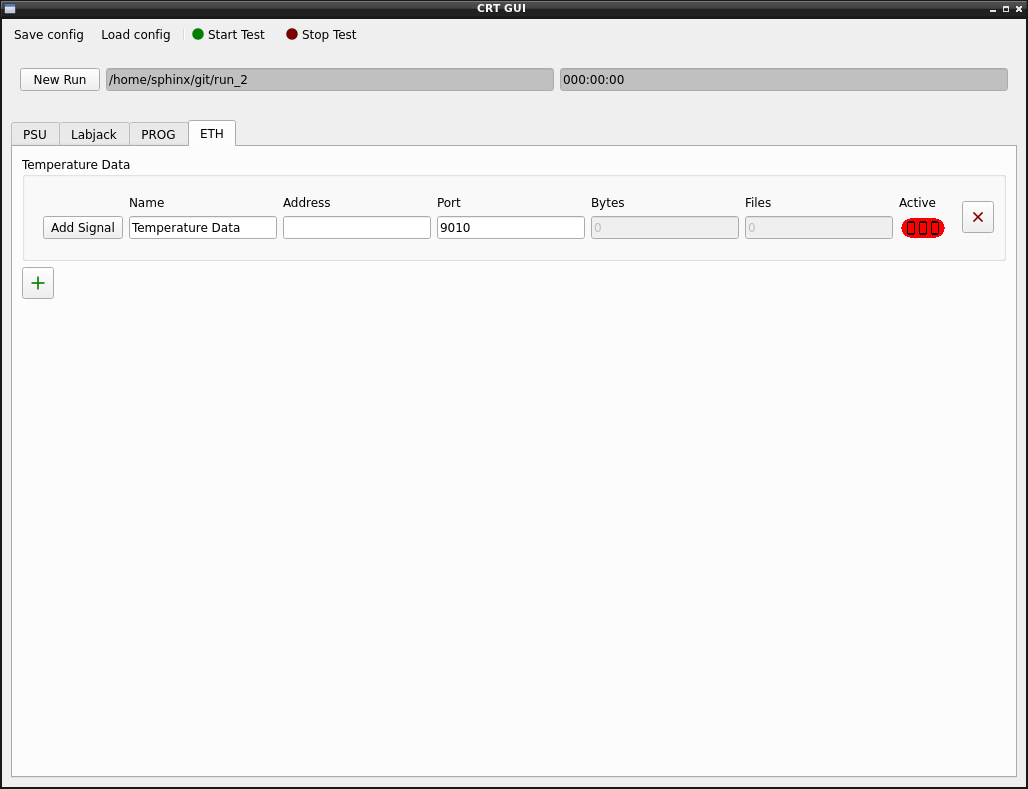
\includegraphics[width=0.9\textwidth]{./8_ETH_example.png}
\caption{An example with a Rohde\&Schwarz 3-channel power supply}
\label{f:eth_example}
	\end{figure}	 
	
	\subsubsection{Manual Creation}	
	\label{c:eth_manual_creation}
	
	The window for manual creation is presented in figure \eqref{f:eth_menu}. In the first row an individual (meaningful) name can be chosen. This is also the folder where the received files are stored later! In the second row the port number is given. At last an arbitrary timeout (in milliseconds) can be specified.
	
	\begin{figure}[H]
	\centering
	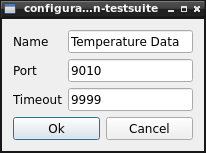
\includegraphics[width=0.4\textwidth]{./8_ETH_menu.png}
	\caption{Creation menu for a power-supply}
	\label{f:eth_menu}
	\end{figure}
	
	\subsubsection{Config Creation}
	
	The ethernet is denoted in the configuration file in the \enquote{ETH} section. All three lines correspond to the manual creation in chapter \ref{c:eth_manual_creation}. 
	
\begin{lstlisting}[caption=PSU Config]
Section PSU
	name=PSU Links
	port=9010
	timeout=9999
	signal=
EndSection
\end{lstlisting}
	
\newpage
\section{Signal Event Mechanism}
\label{c:signal_event_mechanism}

The signal event mechanism allows the user to define interactions between components. For example if a certain event happens in component \textbf{A} it can trigger an action in component \textbf{B}. Signals are added via the \enquote{Add Signal} button in the components window. If no such button is available it means that this component is not able to send any signal.

	\subsection{Usage Example}
	
	If one has a power-supply and a LabJack set up, a signal interaction can be created. The LabJack has a button to add signals (see figure \ref{f:sem_menu}). Here the user can choose what action should be taken if a certain value boundary is crossed. In this case, the power-supply would switch off if a boundary crossing would occur.
	
	\begin{figure}[H]
	\centering
	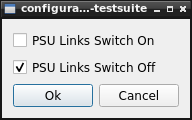
\includegraphics[width=0.3\textwidth]{./5_sem_menu.png}
	\caption{\enquote{Add Signal} menu with available signals}
	\label{f:sem_menu}
	\end{figure}


\newpage
\appendix

\section{Appendix}

\subsection{Diagrams}

\begin{figure}[H]
\centering
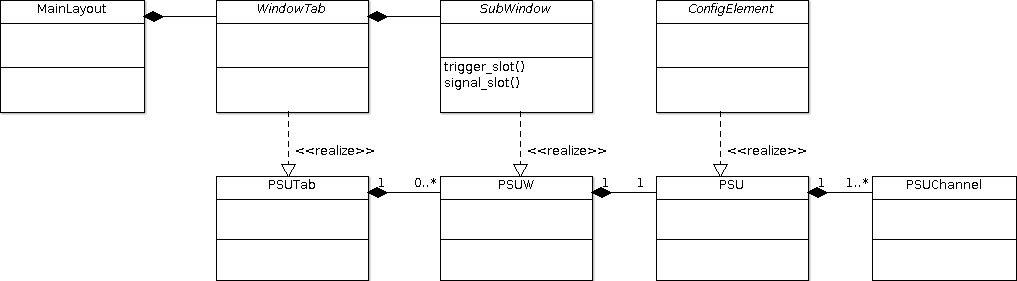
\includegraphics[width=0.9\textwidth]{./A_MainLayout.png}
\caption{UML diagram of the abstract window classes all together down to the component interaction level}
\end{figure}

\begin{figure}[H]
\centering
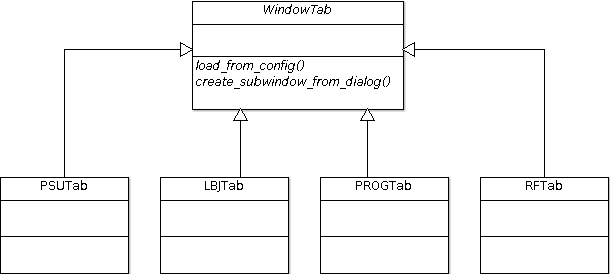
\includegraphics[width=0.9\textwidth]{./A_WindowTabDiagramm.png}
\caption{UML diagram of the abstract WindowTab with the children}
\end{figure}

\begin{figure}[H]
\centering
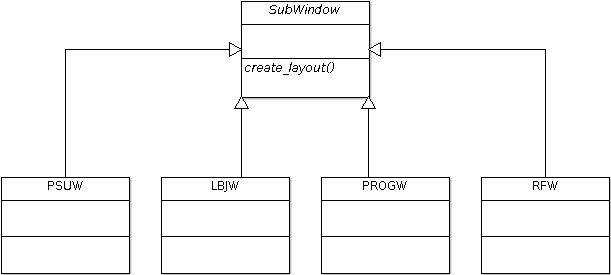
\includegraphics[width=0.9\textwidth]{./A_SubWindowDiagramm.png}
\caption{UML diagram of the abstract SubWindow classes with the children}
\end{figure}

\begin{figure}[H]
\centering
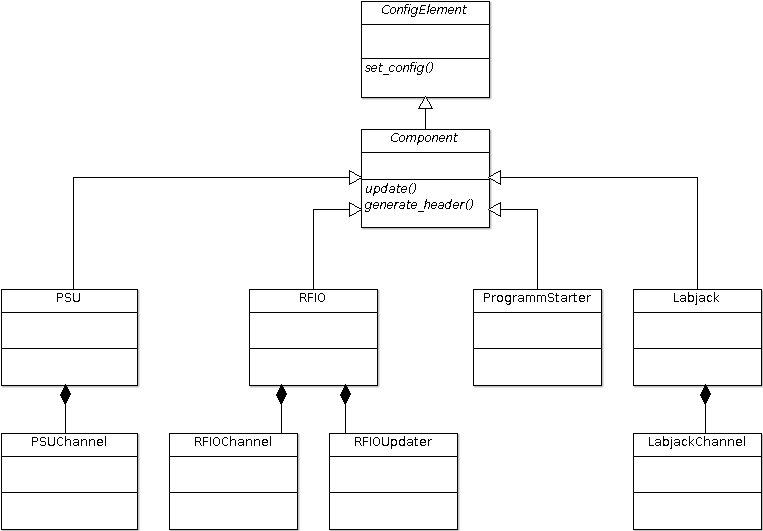
\includegraphics[width=0.9\textwidth]{./A_ComponentDiagramm.png}
\caption{UML diagram of the abstract ConfigElement and Component classes which build up the interface to the real hardware}
\end{figure}

\begin{figure}[H]
\centering
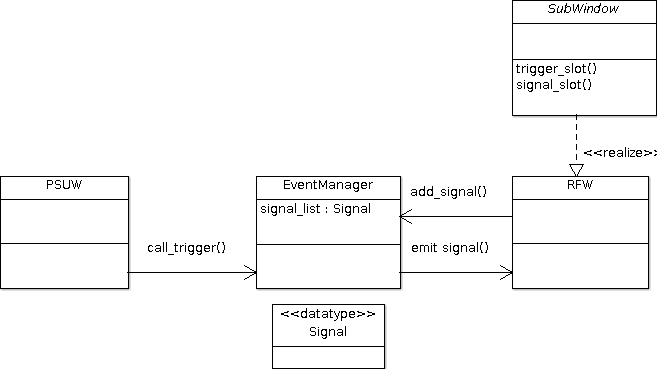
\includegraphics[width=0.9\textwidth]{./A_EventManager.png}
\caption{Signal Event Mechanism described in the \textit{EventManager} and the \textit{SubWindow} with an example}
\label{f:signal_event_mechanism}
\end{figure}

\subsection{Signal Event Mechanism}

To understand the signal event mechanism an overview of the participating classes is presented in figure \ref{f:signal_event_mechanism}. 

\bigbreak

In the \textit{SubWindow} are general cases of signals and corresponding slots defined. The signals can be added to the \textit{EventManger} in the derived \textit{SubWindow} classes. Theses signals are then official and can then be used to trigger actions. Either internally in the program code or externally by adding signals in the GUI via dialog. 

	\subsubsection{Event Manager}
	
	The \textit{EventManger} class object exists only once in the program. It presents an interface to all the other classes to handle signals and slots and especially the interaction between \textit{SubWindows} and their components. For this to work, the signals from the \textit{SubWindow} have to be added to the \textit{EventManager}.
	
		\paragraph{Registered Signal Structure}

		A signal from the \textit{SubWindow}, which is added to the \textit{EventManager}, holds the following properties:
		
\begin{lstlisting}[caption=EventManager.h]
struct RegisteredSignal {
	QString name;
	SignalType st;

	SubWindow *sub;
	void (SubWindow::*sp)(void);
};
\end{lstlisting}

			The name is a descriptive name and should consist of the components name (\textit{cfg\_element\_name}) and info of the action (e.g. turn on, turn off). The signal type is one of the predefined types / actions listed in the \textit{EventManager}. The next two rows are the pointers to find the signal later on and to emit them via the call mechanism.

		\paragraph{Call Mechanism}
		
		To now emit the registered signals and cause an action, the \textit{call\_tigger()} method is used which needs the type of signal to be triggered and a signal list to choose from:
		
\begin{lstlisting}[caption=EventManager.cpp]
void EventManager::call_trigger(enum SignalType st,
const QVector<struct RegisteredSignal*> &signal_list) {

    RegisteredSignal * signal;
    foreach (signal, signal_list)
        if(signal->st == st)
            emit ((signal->sub)->*(signal->sp))();
}
\end{lstlisting}

	\subsubsection{Sub Window}
	
	In the \textit{SubWindow} a general set of signals and slots is available. These can be implemented in the derived classes for easy interaction internally as well as externally. The class holds a signal list with signals which have been added either internal or external. All the available signals are stored in the signal list of the \textit{EventManager}.

		\paragraph{Code Example}

		First, in the derived subclass the used signals have to be registered to inform the \textit{EventManager} (and therefore the outer world) about it. In this example we announce from our power-supply the signals \enquote{on} and \enquote{off}. Which means that our power-supply is listening and will turn itself on or off if one of these signals are emitted:
		
\begin{lstlisting}[caption=PSU.cpp]
PSU::PSU() {
 connect(this, SIGNAL(signal_on()), psu, SLOT(switch_on()));
 connect(this, SIGNAL(signal_off()), psu, SLOT(switch_off()));

 eventManager->add_signal(psu->get_element_name() + " Switch On",
  SignalType::on, this, &SubWindow::signal_on);
 eventManager->add_signal(psu->get_element_name() + " Switch Off",
  SignalType::off, this, &SubWindow::signal_off);
 }
\end{lstlisting}

If one now wants to not only react, but also to trigger other components, the predefined slots have to be used. They can be connected to certain internal class signals. 

For example if we track various sub-voltages on a board via LabJack, we can then connect an off-signal if we cross a set boundary:

\begin{lstlisting}[caption=PSU.cpp]
connect(channel, SIGNAL(boundary_check_failed()),
 this, SLOT(trigger_signal_list()));
\end{lstlisting}

If a voltage now crosses a boundary, all signals that have been added to the signal list are now emitted. The action could be also limited by calling only off-signals with the other slots.

\end{document}